\documentclass[tikz,border=0pt]{standalone}
\usepackage[american]{circuitikz}
\usetikzlibrary{arrows.meta,calc,positioning,decorations.pathmorphing,patterns}
\definecolor{zyloTeal}{HTML}{174A5B}
\definecolor{zyloTealTwo}{HTML}{246B7A}
\definecolor{zyloInk}{HTML}{1F2933}
\definecolor{zyloSoft}{HTML}{EAF4F4}
\definecolor{zyloPaper}{HTML}{F8FAFB}
\definecolor{zyloLine}{HTML}{44606B}
\definecolor{zyloOrange}{HTML}{D97706}
\begin{document}
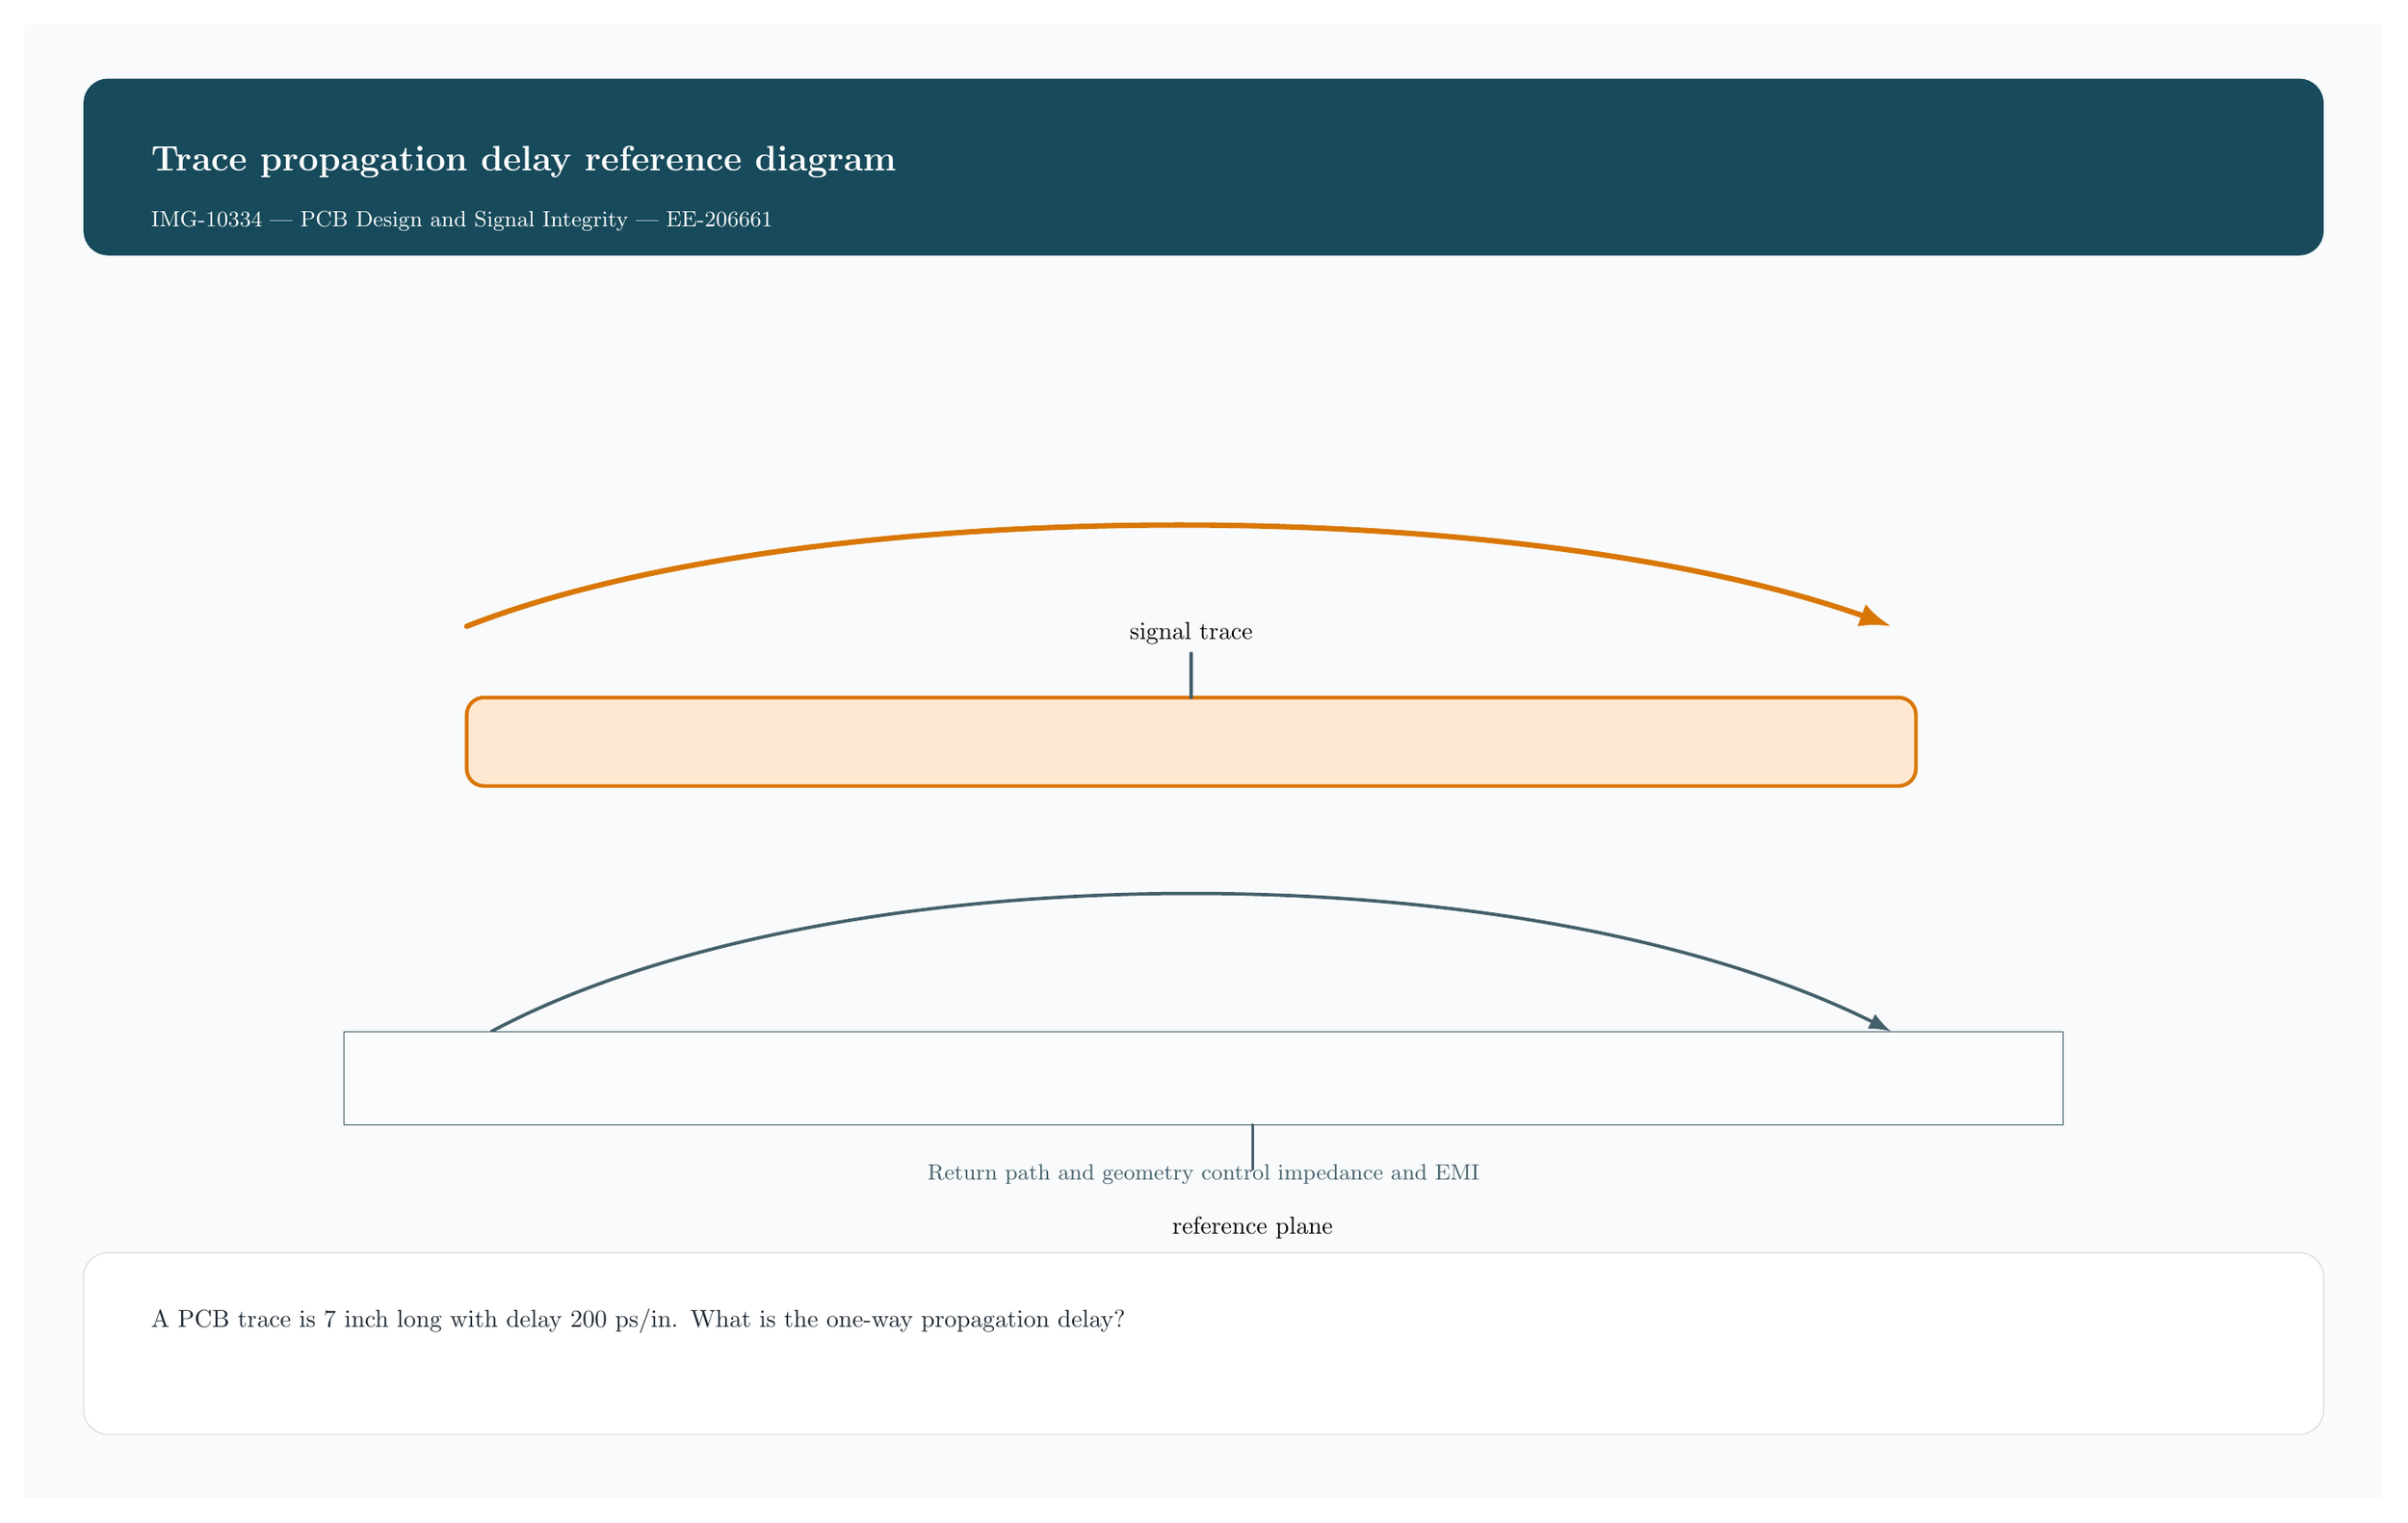
\begin{tikzpicture}[x=1pt,y=-1pt,>=Latex,line cap=round,line join=round]
\path[fill=zyloPaper] (0,0) rectangle (960,600);
\path[fill=zyloTeal,rounded corners=10pt] (24,22) rectangle (936,94);
\node[anchor=west,text=white,font=\bfseries\Large] at (48,56) {Trace propagation delay reference diagram};
\node[anchor=west,text=white!82,font=\small] at (48,80) {IMG-10334 | PCB Design and Signal Integrity | EE-206661};
\tikzset{wire/.style={draw=zyloTeal,line width=2.2pt},thinwire/.style={draw=zyloLine,line width=1.35pt},accent/.style={draw=zyloOrange,line width=2.2pt},box/.style={draw=zyloTealTwo,fill=zyloSoft,line width=1.5pt,rounded corners=8pt}}
\draw[accent,->] (180,245) .. controls (320,190) and (620,190) .. (760,245);
\path[draw=zyloOrange,fill=orange!18,rounded corners=7pt,line width=1.5pt] (180,274) rectangle (770,310);
\draw[thinwire] (475,256) -- (475,274); \node at (475,248) {signal trace};
\draw[thinwire,->] (190,410) .. controls (330,335) and (620,335) .. (760,410);
\path[draw=zyloLine,fill=white!80!zyloSoft] (130,410) rectangle (830,448);
\draw[thinwire] (500,448) -- (500,466); \node at (500,490) {reference plane};
\node[font=\small,text=zyloLine] at (480,468) {Return path and geometry control impedance and EMI};
\path[draw=black!15,fill=white,rounded corners=10pt] (24,500) rectangle (936,574);
\node[anchor=west,text width=860pt,align=left,text=zyloInk,font=\normalsize] at (48,528) {A PCB trace is 7 inch long with delay 200 ps/in. What is the one-way propagation delay?};
\end{tikzpicture}
\end{document}
